\makeatletter
\def\input@path{{ijcs_template/Optimal-Design-layout/}}
\makeatother
\documentclass[ASNA,twocolumn]{USG}

\usepackage{anyfontsize}
\usepackage{amsmath}
\usepackage{amssymb}
\usepackage{booktabs}
\usepackage{multirow}
\usepackage{array}
\usepackage{graphicx}
\usepackage{xcolor}
\usepackage{url}

\graphicspath{{figures/}{ijcs_template/Optimal-Design-layout/images/}{ijcs_template/Optimal-Design-layout/}}

\articletype{RESEARCH ARTICLE}
\received{}
\revised{}
\accepted{}
\journal{International Journal of Communication Systems}
\volume{}
\copyyear{2026}
\startpage{1}
\articledoi{}

\begin{document}

\title{Digital-Twin-Aware Joint Synchronization and Control for Secure UAV Communication Systems}
\transtitle{Digital-Twin-Aware Joint Synchronization and Control for Secure UAV Communication Systems}

\author[1]{Keju Du}
\author[1]{Qianli Di}
\author[1]{Hai Deng}

\authormark{DU, DI, and DENG}
\titlemark{Digital-Twin-Aware Secure UAV Communication}

\address[1]{\orgdiv{College of Computer Science and Technology, }\orgname{Nanjing University of Aeronautics and Astronautics, }%
\orgaddress{\city{Nanjing, }\postcode{211106, }\country{China}}}

\corres{Qianli Di (\email{diqianli@nuaa.edu.cn})}

\keywords{UAV communication | digital twin | physical-layer security | secrecy outage | synchronization control | rollout control}
\transkeywords{UAV communication | digital twin | physical-layer security | secrecy outage | synchronization control | rollout control}

\abstract[ABSTRACT]{Secure unmanned aerial vehicle (UAV) communication often operates with imperfect knowledge of mobile eavesdroppers. Digital twins can maintain such state information, but synchronization consumes resources and stale twins may mislead trajectory, power, and jamming decisions. This paper studies a digital-twin-aware secure UAV communication system with two cooperative UAVs, multiple ground users, a mobile eavesdropper, and budget-limited twin synchronization. We formulate a joint synchronization-control problem and propose an empirical-risk-aware rollout controller that jointly selects synchronization bandwidth, UAV motion, source power, and cooperative jamming power. To quantify risk from twin uncertainty, we fit a secrecy-loss risk estimator with train/calibration/validation separation and use its slack in the rollout score. Multi-seed simulations are conducted on base, hard, and calibrated stress scenarios. The gains are regime-dependent: compared with fixed periodic synchronization, the base scenario yields a modest secrecy-rate increase of 0.0314 with unchanged outage, the hard scenario improves secrecy rate by 0.1626 with nearly unchanged outage, and the 20-seed stress scenario improves secrecy rate from 0.9858 to 1.2540 while reducing outage from 0.6434 to 0.4294 at the calibrated stress threshold $R_{\min}=1.10$. A stress-threshold sweep shows stable secrecy-rate gains, while outage reduction is concentrated in the non-saturated threshold range. Holdout cover rates for the fitted upper bound are 0.9873, 1.0000, and 1.0000 for the base, hard, and stress groups. Additional stress experiments show that the proposed method outperforms SCA-based, no-twin, no-synchronization, and fixed-periodic baselines, while remaining below an oracle-state upper reference. The current implementation is more computationally expensive than rule-based baselines.}

\maketitle

\section{Introduction}
\label{sec:introduction}

Unmanned aerial vehicles (UAVs) have become an important component of flexible wireless communication systems. Compared with fixed terrestrial infrastructure, UAV communication platforms can be rapidly deployed, repositioned according to demand, and used for emergency coverage, temporary networking, surveillance support, aerial relaying, and mission-oriented connectivity \cite{zeng2016uav,mozaffari2019tutorial}. The same mobility and line-of-sight channel characteristics that make UAVs attractive, however, also create security risks. Wireless signals are broadcast by nature, UAV-ground links are often visible over large areas, and adversarial receivers can move to favorable interception locations. Physical-layer security is therefore a natural tool for UAV systems because it directly characterizes secrecy performance from the difference between legitimate and eavesdropping channels \cite{wyner1975wiretap,csiszar1978broadcast}.

A substantial body of work has studied secure UAV communication through trajectory optimization, power allocation, and cooperative jamming. These studies have shown that UAV mobility can be actively exploited to improve secrecy rate by moving the legitimate transmitter closer to intended users and by positioning a friendly jammer to degrade the eavesdropper channel \cite{zhang2019securing,zhong2019cooperative,zhou2018unknown,sun2019aerial}. Most such formulations, however, assume that the controller either knows the relevant channel state or has a fixed uncertainty model. In practical secure UAV operation, the controller may only maintain an estimated state of the eavesdropper through sensing, tracking, network telemetry, or edge-side prediction. This state estimate can be viewed as a digital twin of the adversarial environment.

Digital twins are increasingly discussed as enablers for autonomous wireless networks and UAV networks because they can support simulation, prediction, policy adaptation, and network management before actions are applied to the physical system \cite{kuruvatti2022digital,mcmanus2023digital}. A twin is useful only when it remains sufficiently synchronized with the physical process. Updating the twin consumes sensing, control, or communication resources; delayed or failed updates leave the controller with stale information. This creates a control problem that is different from conventional trajectory-only optimization: the system must decide not only where the UAVs should move and how much power they should use, but also when and how strongly the twin should be synchronized.

This paper studies this coupled problem for secure UAV communication. We consider two cooperative UAVs, multiple ground users, a mobile eavesdropper, and a limited synchronization budget. One UAV serves as the confidential transmitter, while the other provides cooperative jamming. The controller observes a digital-twin state of the eavesdropper and must choose synchronization bandwidth, UAV motion, source power, and jamming power at every time slot. The objective is to improve average secrecy rate, reduce secrecy outage, and avoid unsafe decisions caused by stale or uncertain twin states. Figure~\ref{fig:framework} summarizes the resulting closed-loop control structure.

\begin{figure*}[t]
\centering
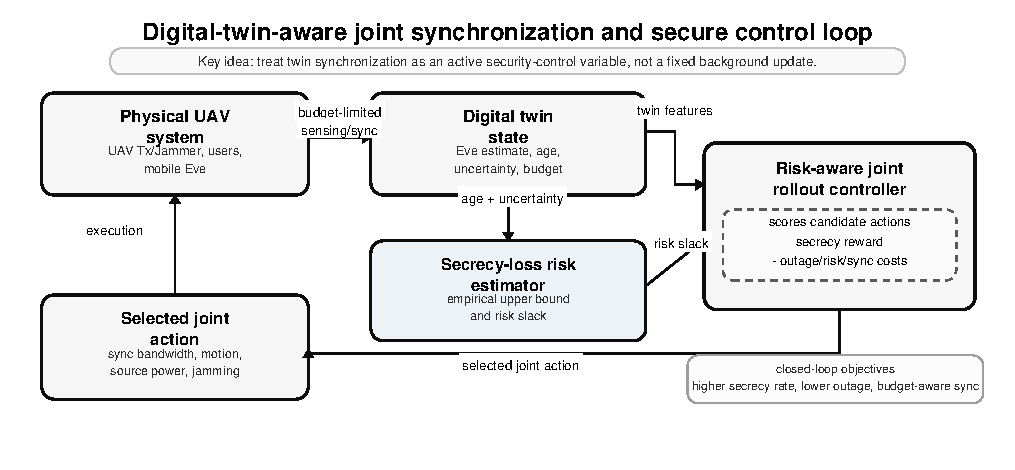
\includegraphics[width=0.92\textwidth]{dt_uav_joint_sync_secure_control_loop.pdf}
\caption{Digital-twin-aware joint synchronization and secure control loop. The physical UAV system updates the digital-twin state through budget-limited sensing and synchronization. The risk-aware rollout controller uses twin features and secrecy-risk slack to jointly select synchronization, UAV motion, source-power, and jamming-power actions.}
\label{fig:framework}
\end{figure*}

The main challenge is that synchronization and communication control are strongly coupled over time. A fixed-period synchronization rule is simple and inexpensive, but it does not react to secrecy risk, remaining budget, or the future value of information. A security-risk trigger can synchronize under dangerous states, but it still separates synchronization from motion and power decisions. A local optimization method can improve per-slot actions, but it may be shortsighted when future twin quality and outage penalties matter. A learning-based controller can be fast at inference time, but the coupled action space makes training difficult under limited data and computation.

To address these issues, we propose an empirical-risk-aware joint rollout controller, denoted as \texttt{rollout\_joint}. The controller enumerates feasible synchronization bandwidths, UAV movements, source power levels, and jamming power levels, and evaluates them using a finite-horizon score. The score combines predicted secrecy reward, outage penalty, synchronization cost, twin-quality terms, and an empirical secrecy-loss penalty. The fitted risk estimator is learned from simulated trajectories using a holdout procedure and is used as an empirical upper bound on secrecy loss induced by twin uncertainty. We emphasize that this estimator is an in-policy, simulation-validated diagnostic; it is not claimed as a finite-sample safety guarantee or a universal proof under arbitrary distribution shift.

The contributions of this paper are as follows:
\begin{enumerate}
    \item We formulate a digital-twin-aware secure UAV communication problem in which twin synchronization, secrecy rate, secrecy outage, UAV mobility, transmit power, and cooperative jamming are optimized in a unified control loop.
    \item We design an empirical-risk-aware rollout controller that jointly selects synchronization and communication-control actions, rather than treating twin updates as a separate rule-based module.
    \item We construct a holdout-fitted secrecy-loss risk estimator and report empirical upper-bound coverage on held-out trajectories from base, hard, and calibrated stress scenarios.
    \item We provide a multi-seed simulation study with rule-based baselines, SCA baselines, a lightweight PPO diagnostic run, oracle references, ablations, runtime analysis, and a small exact-DP sanity check. In the calibrated stress scenario, the proposed controller improves average secrecy rate over periodic synchronization by 0.2683 and reduces secrecy outage by 0.2141.
\end{enumerate}

The rest of this paper is organized as follows. Section~\ref{sec:related} reviews related work. Section~\ref{sec:model} presents the system model and metrics. Section~\ref{sec:method} describes the risk estimator and joint rollout method. Section~\ref{sec:experiments} reports the experimental results. Section~\ref{sec:discussion} discusses interpretation and limitations. Section~\ref{sec:conclusion} concludes the paper.

\section{Related Work}
\label{sec:related}

\subsection{UAV communication and FANET systems}

UAV-enabled wireless communication has been widely studied because aerial platforms can provide on-demand coverage, relay support, flexible topology control, and rapid deployment in infrastructure-limited scenarios \cite{zeng2016uav,mozaffari2019tutorial}. Channel geometry, altitude, energy constraints, mobility, and interference are central design factors. The altitude-dependent coverage model in \cite{alhourani2014optimal}, for example, illustrates that UAV placement has a direct effect on link quality. FANET research further considers multiple UAVs with fast topology changes and mission-oriented networking constraints \cite{lakew2020fanet}. Within the target journal, energy-efficient FANET routing \cite{oubbati2019ecad}, mission-oriented UAV swarm fault tolerance \cite{wang2021fault}, and UAV simulation tools \cite{jiang2024simulation} show that communication-system-level modeling and reproducible simulation remain important research directions.
Recent IJCS work has also considered UAV-assisted anti-jamming and proactive handoff with deep-learning support \cite{unnisa2023antijamming}, which is close to the present paper's emphasis on adversarial wireless environments.

The present work is related to this literature but has a different focus. We do not study multi-hop FANET routing or swarm task allocation. Instead, we study a secure communication control problem in which two cooperative UAVs must serve users and jam an eavesdropper while maintaining a synchronized digital twin of the adversarial state.

\subsection{Physical-layer security for UAV communications}

Physical-layer security originates from information-theoretic secrecy models such as the wiretap channel \cite{wyner1975wiretap} and broadcast channels with confidential messages \cite{csiszar1978broadcast}. In UAV systems, secrecy depends heavily on geometry because UAV mobility changes the legitimate and eavesdropping channel gains. Joint trajectory and power optimization has therefore become a common approach. Zhang et al. \cite{zhang2019securing} optimized UAV trajectory and transmit power for secure UAV communication. Cooperative jamming has also been introduced to improve secrecy; Zhong et al. \cite{zhong2019cooperative} studied a two-UAV setting with a transmitter UAV and a jammer UAV, while Zhou et al. \cite{zhou2018unknown} considered a friendly UAV jammer when the eavesdropper location is uncertain. Sun et al. \cite{sun2019aerial} further examined aerial cooperative jamming with joint trajectory and power control.

Recent work has moved toward more realistic secure UAV settings with sensing, edge computing, channel uncertainty, and learning-based optimization. Wei et al. \cite{wei2024isncsecureuav} considered an integrated sensing, navigation, and communication framework for a secure UAV network with a mobile aerial eavesdropper. Mao et al. \cite{mao2023secureuavmec} and Lu et al. \cite{lu2024securemaritimemec} studied secure UAV-assisted MEC systems with coupled trajectory, resource, and security constraints. Ding et al. \cite{ding2024ddqnuavmec} used a DDQN-based method for trajectory and resource optimization in UAV-aided MEC secure communications, while Liu et al. \cite{liu2024secureisacuav} and Chen et al. \cite{chen2025covertuavmec} addressed recent ISAC-UAV and covert UAV-MEC security problems.

These works motivate our use of trajectory, transmit power, and jamming power as control variables, and they provide the most relevant recent context for the baselines in this paper. The key distinction is the information state. Rather than assuming a fixed eavesdropper state, a one-shot uncertainty set, or an MEC/offloading objective, we model a digital twin whose quality evolves according to synchronization decisions. Consequently, secrecy performance depends not only on the physical trajectory and power allocation, but also on whether the controller has recently synchronized the twin. Directly importing the DDQN or SCA implementations from these papers would change the state, action, constraints, and reward definitions; we therefore compare against matched in-simulator rollout, rule-based, and SCA-style diagnostic baselines, and we state this scope explicitly in the experiments.

\subsection{Digital twins and information freshness}

Digital twins have been proposed as a means to support intelligent wireless systems, network automation, and data-driven control. Surveys on 6G and wireless digital twins discuss their role in modeling physical network behavior, supporting closed-loop control, and reducing the risk of deploying untested policies \cite{kuruvatti2022digital}. For UAV networks, digital-twin-enabled domain adaptation has been identified as a promising direction for zero-touch control, simulation-to-real transfer, and robust policy evaluation \cite{mcmanus2023digital}.
Recent digital-twin communication work is closer to the present setting. Li et al. \cite{li2023adaptivedt} studied adaptive digital twins for UAV-assisted integrated sensing, communication, and computation networks. Yang et al. \cite{yang2024syncdelay} optimized synchronization delay for wireless digital twins, and a related joint communication-computation framework for digital twins over wireless networks was developed in \cite{yang2024jointdt}. These papers emphasize that synchronization and communication/computation resources must be optimized jointly, which aligns with the motivation of this paper.

The synchronization aspect of our problem is also related to age of information (AoI), which measures the freshness of status updates. Early AoI work showed that update frequency should be optimized rather than simply maximized, because network resources and queueing effects create tradeoffs \cite{kaul2012aoi}. Vehicular-network AoI studies reached similar conclusions for mobile systems \cite{kaul2011vehicular}. Our setting shares the same core idea that stale information is harmful, but the performance target is different: we optimize secrecy rate and secrecy outage under a limited synchronization budget, not only information freshness.

\subsection{Optimization, reinforcement learning, and empirical risk estimation}

Many UAV secrecy problems are nonconvex because channel gains, trajectory variables, and power decisions are coupled. Successive convex approximation and alternating optimization are therefore widely used in recent secure UAV optimization studies \cite{mao2023secureuavmec,wei2024isncsecureuav,lu2024securemaritimemec,liu2024secureisacuav}, with convex optimization providing the standard mathematical foundation \cite{boyd2004convex}. In this paper, the SCA-based baselines are matched local-optimization diagnostics under either deployable twin information or oracle eavesdropper information; they are not presented as a reproduction of a particular external paper, and Boyd's text is cited only as background for the convex-optimization machinery.

Reinforcement learning is another natural approach for sequential control. PPO \cite{schulman2017ppo} is a widely used policy-gradient method and is included as a lightweight learning-based diagnostic in our experiments. We do not claim that PPO is intrinsically unsuitable; our result only evaluates a limited-training run under the same simulator.

Finally, our secrecy-loss risk estimator uses a simple residual-calibration idea: fit a loss model, add a calibration residual quantile, and validate the resulting upper bound on held-out simulator traces. We do not present it as a contribution to formal predictive inference, nor do we claim a finite-sample coverage theorem under arbitrary deployment conditions. It is a holdout-fitted empirical upper bound that is calibrated and validated on simulated trajectory distributions. This conservative interpretation is important for avoiding overstatement of the estimator's scope.

\section{System Model}
\label{sec:model}

\subsection{Network and mobility model}

We consider a time-slotted UAV-assisted secure communication system indexed by $t=0,1,\ldots,T-1$. The service area contains a set of ground users $\mathcal{U}$, two cooperative UAVs, and a mobile eavesdropper Eve. UAV 1 acts as the confidential transmitter and UAV 2 acts as a cooperative jammer. The UAV altitude is fixed at $H$, while horizontal positions evolve in a two-dimensional rectangular area. The horizontal positions of UAV 1, UAV 2, user $u$, and Eve at slot $t$ are denoted by $\mathbf{q}_1(t)$, $\mathbf{q}_2(t)$, $\mathbf{w}_u$, and $\mathbf{e}(t)$, respectively.

The UAVs choose movement commands from a finite action set such as staying, moving up, down, left, or right. Each non-stationary movement changes the horizontal position by the configured step size and is clipped to the service region. Eve follows an adaptive mobile process in the simulator with bounded speed and random motion perturbations. The controller does not directly observe $\mathbf{e}(t)$ at all times; it observes a digital-twin estimate described below.

\subsection{Air-to-ground channel and secrecy rate}

For a horizontal transmitter-receiver pair $(\mathbf{x},\mathbf{y})$, the three-dimensional distance is
\begin{equation}
    d(\mathbf{x},\mathbf{y})=
    \sqrt{\|\mathbf{x}-\mathbf{y}\|_2^2+H^2}.
\end{equation}
The large-scale channel gain used by the simulator is
\begin{equation}
    g(\mathbf{x},\mathbf{y})=
    \frac{\beta_0}{d(\mathbf{x},\mathbf{y})^\alpha}\eta(\mathbf{x},\mathbf{y}),
\end{equation}
where $\beta_0$ is a reference gain, $\alpha$ is the path-loss exponent, and $\eta(\mathbf{x},\mathbf{y})$ is an optional probabilistic line-of-sight attenuation factor. In the final scenarios, the simulator uses a probabilistic LoS model with LoS and NLoS attenuation parameters from the configuration files.

For a selected user $u$, source power $p_s(t)$, and jamming power $p_j(t)$, the legitimate rate and eavesdropping rate are
\begin{align}
    R_b(t,u) &=
    \log_2\left(1+
    \frac{p_s(t)g(\mathbf{q}_1(t),\mathbf{w}_u)}
    {\sigma_n^2+\xi p_j(t)g(\mathbf{q}_2(t),\mathbf{w}_u)}
    \right), \\
    R_e(t,u) &=
    \log_2\left(1+
    \frac{p_s(t)g(\mathbf{q}_1(t),\mathbf{e}(t))}
    {\sigma_n^2+p_j(t)g(\mathbf{q}_2(t),\mathbf{e}(t))}
    \right),
\end{align}
where $\sigma_n^2$ is noise power and $\xi$ models residual interference from the friendly jammer at the legitimate receiver. The instantaneous secrecy rate for user $u$ is
\begin{equation}
    R_s(t,u)=\left[R_b(t,u)-R_e(t,u)\right]^+.
\end{equation}
The simulator serves the user with the best resulting secrecy metric at each slot, and the reported slot secrecy rate is denoted by $R_s(t)$. The average secrecy rate is
\begin{equation}
    \bar{R}_s=\frac{1}{T}\sum_{t=0}^{T-1}R_s(t).
\end{equation}

\subsection{Digital twin and synchronization}

The controller maintains a digital twin of Eve's state. The twin contains an estimated Eve position $\hat{\mathbf{e}}(t)$, an age-of-information value $A(t)$, an uncertainty scale $\sigma(t)$, and derived quality and badness indicators. If no synchronization is applied, the twin prediction evolves forward and its age and uncertainty increase. If synchronization is requested with bandwidth $b_t>0$, a portion of the finite synchronization budget is consumed. The update may be delayed by the configured number of slots and may fail with a configured probability. Higher bandwidth reduces measurement noise but consumes more budget.

The synchronization decision is therefore a value-of-information decision. Synchronizing too often can exhaust the budget and reduce future flexibility. Synchronizing too rarely can make the controller act on a stale eavesdropper estimate, leading to optimistic secrecy predictions and increased outage.

\subsection{Action space and objective metrics}

At each slot the controller selects
\begin{equation}
    a_t=(b_t,m_{1,t},m_{2,t},p_s(t),p_j(t)),
\end{equation}
where $b_t$ is the synchronization bandwidth, $m_{1,t}$ and $m_{2,t}$ are the UAV movement commands, and $p_s(t)$ and $p_j(t)$ are source and jamming power levels. The feasible sets are finite in the simulator. The synchronization bandwidth set includes zero and several positive bandwidth levels, while power levels are selected from configured discrete sets.

We evaluate policies using five metrics:
\begin{itemize}
    \item average secrecy rate $\bar{R}_s$, where higher is better;
    \item secrecy outage probability
    \begin{equation}
        P_{\mathrm{out}}=\frac{1}{T}\sum_{t=0}^{T-1}\mathbb{I}\{R_s(t)<R_{\min}\},
    \end{equation}
    where lower is better;
    \item average synchronization cost, which measures synchronization-budget consumption;
    \item empirical upper-bound cover rate, which measures whether the fitted secrecy-loss upper bound covers realized loss on the evaluated holdout traces;
    \item runtime per slot, which measures decision-time cost.
\end{itemize}

The final calibrated stress scenario uses $R_{\min}=1.10$ as its main operating point. This value is treated as a feasible but non-trivial service threshold selected after a pilot feasibility sweep: the earlier threshold made every evaluated method remain in outage, which removed the ability to compare methods by outage probability. It is not used as a method-tuned optimum. Since outage conclusions can depend on this threshold, claims about outage reduction in the stress scenario should be interpreted at the calibrated operating point and checked against the explicit $R_{\min}$ sensitivity sweep. The base and hard scenarios retain their configured thresholds and remain useful for testing whether the controller is competitive under different operating regimes.

\subsection{Twin-induced secrecy loss}

Let $\widehat{R}_s(t)$ be the secrecy value predicted from the twin state and $R_s(t)$ be the realized secrecy value under the true Eve state. We define the realized secrecy loss as a nonnegative measure of twin optimism,
\begin{equation}
    L(t)=\left[\widehat{R}_s(t)-R_s(t)\right]^+.
\end{equation}
The controller uses a fitted upper bound $\widehat{L}_{\mathrm{ub}}(t)$ constructed from twin age, predicted error radius, uncertainty scale, synchronization delay, and failure probability. A candidate action is considered safer when its predicted secrecy margin exceeds the required threshold plus this empirical upper bound. This produces a risk-estimator slack term used by the proposed controller.

\section{Proposed Method}
\label{sec:method}

\subsection{Design rationale}

The proposed method is built around two observations. First, synchronization is not an isolated maintenance operation. Its value depends on how the updated twin will change motion, source-power, and jamming decisions over the next few slots. Second, a high twin-predicted secrecy rate can be misleading when the twin is stale or uncertain. The controller should therefore prefer actions that are good under the twin and also have sufficient margin against twin-induced secrecy loss.

We implement this idea through an empirical-risk-aware rollout controller. The rollout controller searches over joint synchronization-control actions and evaluates their short-horizon consequences. The fitted risk estimator supplies a penalty and discourages candidate actions whose predicted secrecy margin is not supported by the empirical upper bound.

\subsection{Holdout-fitted secrecy-loss risk estimator}

The secrecy-loss risk estimator computes an empirical upper bound on $L(t)=[\widehat{R}_s(t)-R_s(t)]^+$. The fitted model uses features derived from the digital twin:
\begin{equation}
    \phi(t)=
    [1,A(t),\hat{d}_e(t),\sigma(t),D_{\mathrm{sync}},p_{\mathrm{fail}},\ldots],
\end{equation}
where $A(t)$ is twin age, $\hat{d}_e(t)$ is the predicted error radius, $\sigma(t)$ is the uncertainty scale, $D_{\mathrm{sync}}$ is synchronization delay, and $p_{\mathrm{fail}}$ is failure probability. Interaction features such as age-radius and radius-uncertainty products are also used in the implementation.

The fitted loss model has the form
\begin{equation}
    \widehat{L}(t)=\left[\theta^\mathsf{T}\phi(t)\right]^+.
\end{equation}
A residual quantile from a held-out calibration split is added to obtain
\begin{equation}
    \widehat{L}_{\mathrm{ub}}(t)=\widehat{L}(t)+c_{\mathrm{cal}},
\end{equation}
where $c_{\mathrm{cal}}$ is determined on held-out calibration traces. The construction uses the practical idea of residual calibration, but the claim made here is deliberately narrower than a formal distribution-free coverage theorem: the paper reports empirical holdout coverage on simulated trajectories drawn from the evaluated policy and scenario distributions. The validation points are time-correlated trajectory samples, and the estimator is coupled to the policy that uses its slack.

For a candidate action, let $\widehat{M}(t)$ be the predicted secrecy margin relative to the outage threshold. The risk-estimator slack is
\begin{equation}
    S_{\mathrm{risk}}(t)=\widehat{M}(t)-\rho-\widehat{L}_{\mathrm{ub}}(t),
\end{equation}
where $\rho$ is an additional safety margin. Negative slack means that the twin-predicted margin is not large enough after accounting for estimated secrecy loss.

\subsection{Joint rollout action scoring}

At each slot, \texttt{rollout\_joint} constructs a candidate set $\mathcal{A}_t$ from synchronization bandwidths, movement pairs, and power levels. Each candidate action is evaluated by applying a one-step prediction and then a finite-horizon rollout. The immediate score is
\begin{align}
    r_{\mathrm{score}}(s_t,a_t) =
    &\ \widehat{R}_s(t)
    -\lambda_{\mathrm{out}}\widehat{I}_{\mathrm{out}}(t)
    -\lambda_{\mathrm{sync}} b_t
    -\lambda_{\mathrm{pow}}(p_s(t)+p_j(t)) \nonumber \\
    &-\lambda_{\mathrm{risk}}[ -S_{\mathrm{risk}}(t)]^+
    -\lambda_{\mathrm{bad}}B_{\mathrm{twin}}(t),
\end{align}
where $\widehat{I}_{\mathrm{out}}(t)$ is the predicted outage indicator, $B_{\mathrm{twin}}(t)$ is a twin-badness term, and the $\lambda$ coefficients are specified in the scenario configuration. The implementation keeps the legacy configuration key \texttt{lambda\_certificate}, but it is interpreted as the empirical risk-estimator penalty weight. The controller then selects
\begin{equation}
    a_t^\star=\arg\max_{a_t\in\mathcal{A}_t}
    \left\{
    r_{\mathrm{score}}(s_t,a_t)+\gamma V_H(s_{t+1})
    \right\},
\end{equation}
where $\gamma$ is the rollout discount factor and $V_H$ is the approximate value of the remaining rollout horizon. Candidate pruning is used to make the search tractable.

\begin{algorithm}[t]
\caption{Empirical-risk-aware joint rollout controller}
\label{alg:rollout}
\begin{algorithmic}[1]
\State Observe twin state, remaining synchronization budget, UAV states, and pending updates.
\State Build feasible synchronization, movement, source-power, and jamming-power candidates.
\For{each candidate action $a_t\in\mathcal{A}_t$}
    \State Predict the next twin state and physical control effect.
    \State Compute predicted secrecy rate, outage indicator, and risk-estimator slack.
    \State Evaluate immediate risk-aware score.
    \State Estimate finite-horizon rollout value with pruned successor candidates.
\EndFor
\State Select the action with the largest immediate-plus-rollout score.
\State Apply the selected action in the simulator and update pending synchronization state.
\end{algorithmic}
\end{algorithm}

\subsection{Baselines and diagnostic variants}

The experiments compare \texttt{rollout\_joint} with several baselines.

\texttt{periodic} synchronizes at a fixed period and uses greedy communication control. It is simple, stable, and computationally inexpensive. \texttt{security\_risk} triggers synchronization with a weighted score based on age, uncertainty, predicted margin, and budget pressure. \texttt{security\_margin} uses the empirical risk margin to trigger synchronization when the twin-predicted secrecy margin appears insufficient. \texttt{decoupled} separates synchronization from motion and power control.

The SCA baselines represent local optimization inspired by recent secure UAV formulations that use successive convex approximation or alternating optimization for coupled trajectory, resource, and security variables \cite{mao2023secureuavmec,wei2024isncsecureuav,lu2024securemaritimemec,liu2024secureisacuav}; the general convex-optimization reference \cite{boyd2004convex} is used only for background. \texttt{sca\_twin} uses deployable twin information, while \texttt{sca\_oracle} uses true Eve information in the score and is therefore diagnostic. We also include a lightweight PPO diagnostic run following the PPO policy-gradient paradigm \cite{schulman2017ppo}. It is trained for 200 episodes to test whether an inexpensive learning baseline can make progress in this coupled action space; it is not treated as an extensively tuned DRL baseline.

The strengthening suite includes additional diagnostic variants. \texttt{oracle\_sync} uses the true Eve state inside the rollout score and is treated as an upper-reference method. \texttt{rollout\_fixed\_periodic} keeps rollout motion and power search but replaces adaptive synchronization with fixed periodic synchronization. \texttt{no\_twin} disables effective twin prediction, and \texttt{rollout\_no\_sync} disables synchronization while keeping rollout search. These variants identify whether the proposed gain comes from rollout search alone or from the joint use of synchronization, twin prediction, and empirical-risk-aware scoring.

\subsection{Computational implications}

The proposed method is more expensive than rule-based policies because it enumerates a joint action space and performs finite-horizon lookahead. This is a deliberate tradeoff: the method is designed to test whether joint synchronization-control optimization improves secrecy and outage, not to minimize inference latency. Runtime is therefore reported as a first-class experimental metric. Deployment would require either edge-assisted execution, a slower decision timescale, or future acceleration through learned value approximators, parallel candidate evaluation, or stronger pruning.

\section{Experiments}
\label{sec:experiments}

\subsection{Experimental protocol}

All numerical results reported in this section are generated by the project simulator and stored under \texttt{results/final\_2026-05-12/}. No synthetic or hand-adjusted data are introduced in the manuscript. The main experiment evaluates three holdout-fitted scenarios:
\begin{itemize}
    \item \texttt{paper\_base\_holdoutfit}: 120-slot episodes, synchronization budget 28, Eve speed noise standard deviation 0.8, and outage threshold 2.55;
    \item \texttt{paper\_hard\_holdoutfit}: 140-slot episodes, synchronization budget 22, Eve speed noise standard deviation 1.0, and outage threshold 2.72;
    \item \texttt{scenario\_stress\_holdoutfit}: 160-slot episodes, synchronization budget 19, Eve speed noise standard deviation 1.2, and calibrated outage threshold 1.10.
\end{itemize}
The main multi-seed table uses 20 seeds and compares \texttt{rollout\_joint}, \texttt{periodic}, \texttt{security\_risk}, and \texttt{security\_margin}. Additional stress-scenario studies use the same holdout-fitted stress configuration for SCA baselines, PPO, and strengthening ablations.

The primary metrics are average secrecy rate, secrecy outage probability, average synchronization cost, certificate cover rate, and runtime per slot. Higher secrecy rate is better, while lower outage and lower runtime are better. Confidence intervals are computed by the experiment scripts through bootstrap aggregation across seeds. Paired comparisons use matching random seeds for the compared methods.

\subsection{Main 20-seed results}

Table~\ref{tab:main_results} and Figure~\ref{fig:main_results} summarize the main 20-seed results. Across all three scenarios, \texttt{rollout\_joint} achieves the highest average secrecy rate among the four deployable methods. The gain is small in the base scenario, larger in the hard scenario, and strongest in the calibrated stress scenario.

\begin{table*}[t]
\centering
\caption{Main 20-seed results from \texttt{scheme\_c\_readiness\_20seed/main\_table.csv}.}
\label{tab:main_results}
\begin{tabular}{llrrrrr}
\toprule
Scenario & Method & Runs & Secrecy rate & Outage & Sync cost & Runtime ms/slot \\
\midrule
\multirow{4}{*}{Base} 
& rollout\_joint & 20 & 1.6429 & 0.8913 & 0.2018 & 1265.75 \\
& periodic & 20 & 1.6115 & 0.8913 & 0.1500 & 99.65 \\
& security\_risk & 20 & 1.4996 & 0.8896 & 0.0399 & 100.01 \\
& security\_margin & 20 & 0.6913 & 0.8967 & 0.2329 & 101.21 \\
\midrule
\multirow{4}{*}{Hard}
& rollout\_joint & 20 & 1.4429 & 0.9482 & 0.1032 & 1262.04 \\
& periodic & 20 & 1.2803 & 0.9496 & 0.1571 & 97.89 \\
& security\_risk & 20 & 1.2508 & 0.9432 & 0.0389 & 97.77 \\
& security\_margin & 20 & 0.4878 & 0.9657 & 0.1569 & 98.05 \\
\midrule
\multirow{4}{*}{Stress}
& rollout\_joint & 20 & 1.2540 & 0.4294 & 0.1098 & 1295.63 \\
& periodic & 20 & 0.9858 & 0.6434 & 0.1187 & 98.54 \\
& security\_risk & 20 & 0.8680 & 0.7003 & 0.0356 & 99.04 \\
& security\_margin & 20 & 0.6447 & 0.7856 & 0.1186 & 98.60 \\
\bottomrule
\end{tabular}
\end{table*}

\begin{figure*}[t]
\centering
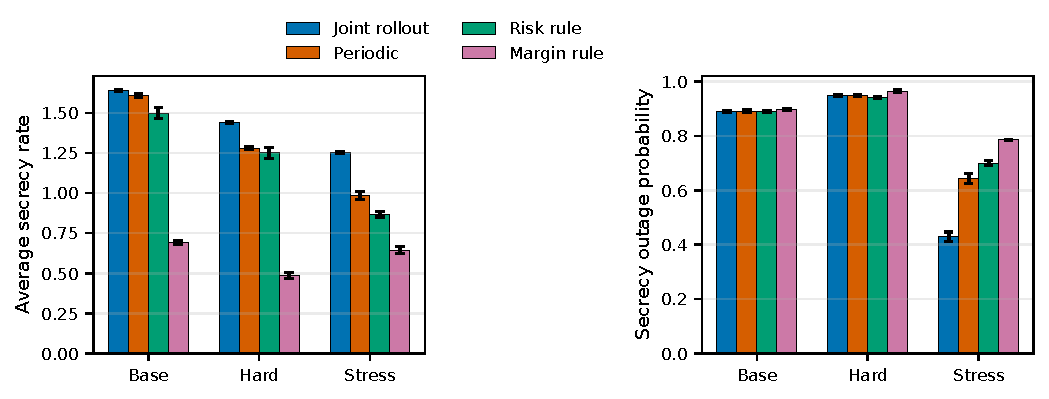
\includegraphics[width=0.92\textwidth]{main_results_secrecy_outage.pdf}
\caption{Average secrecy rate and secrecy outage probability in the main 20-seed experiments. Error bars show the confidence intervals exported by the experiment scripts.}
\label{fig:main_results}
\end{figure*}

In the base scenario, \texttt{rollout\_joint} improves average secrecy rate over \texttt{periodic} by 0.0314, but both methods have the same outage probability. This indicates that the base scenario is not where the proposed method should be oversold; the fixed-period baseline is already strong under this operating condition. In the hard scenario, the secrecy-rate gain increases to 0.1626 with a small outage reduction of 0.0014. In the stress scenario, \texttt{rollout\_joint} increases average secrecy rate from 0.9858 to 1.2540 and reduces outage from 0.6434 to 0.4294 relative to \texttt{periodic}. The paired comparison file reports 20/20 secrecy-rate wins against \texttt{periodic}, \texttt{security\_risk}, and \texttt{security\_margin} in the stress scenario.

\subsection{Certificate validation}

Table~\ref{tab:certificate} and Figure~\ref{fig:certificate} report the holdout certificate validation results. The validation cover rates are above the target 0.95 level for all groups. The base validation group has cover rate 0.9873, while the hard and stress groups both reach 1.0000. The aggregate validation cover rate is 0.9964.

\begin{table}[t]
\centering
\caption{Holdout certificate validation from \texttt{scheme\_c\_holdout/holdout\_summary.csv}.}
\label{tab:certificate}
\begin{tabular}{llrr}
\toprule
Split & Scenario & Cover rate & Avg. realized loss \\
\midrule
validation & base & 0.9873 & 0.5075 \\
validation & hard & 1.0000 & 0.6568 \\
validation & stress & 1.0000 & 0.6916 \\
validation & all & 0.9964 & 0.6279 \\
\bottomrule
\end{tabular}
\end{table}

\begin{figure}[t]
\centering
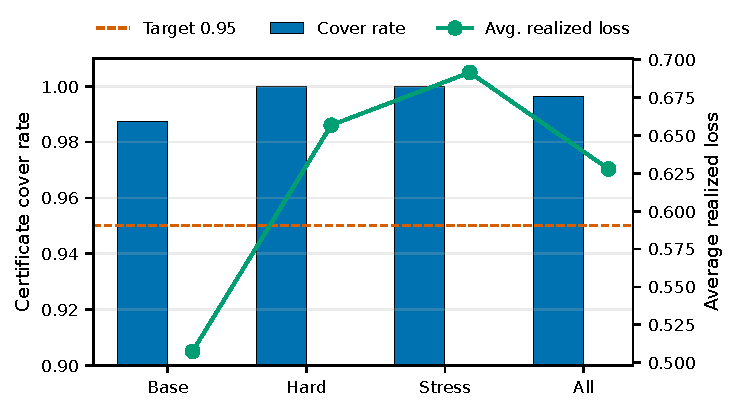
\includegraphics[width=0.98\linewidth]{certificate_validation.pdf}
\caption{Holdout validation cover rates and average realized secrecy loss. The dashed line marks the 0.95 target cover rate.}
\label{fig:certificate}
\end{figure}

These results justify using the certificate as a conservative in-policy risk signal for the evaluated policies and scenarios. They do not justify claiming universal safety under arbitrary environment changes. If the Eve mobility model, channel model, or policy distribution changes substantially, the certificate should be refitted or revalidated.

\subsection{SCA and PPO baselines}

Table~\ref{tab:stress_baselines} reports additional stress-scenario baselines under the same holdout-fitted configuration. The SCA results show that local optimization is not sufficient in this setting. \texttt{sca\_oracle} obtains secrecy rate 1.2126, close to \texttt{rollout\_joint}'s 1.2558, but its outage probability is much worse (0.8125 versus 0.4200). This indicates that improving average secrecy alone does not guarantee reliable secure service. The deployable \texttt{sca\_twin} baseline performs poorly, with secrecy rate 0.4677 and outage 0.8225.

\begin{table*}[t]
\centering
\caption{Stress holdout-fitted SCA and PPO baselines. Values are from the corresponding \texttt{main\_table.csv} files.}
\label{tab:stress_baselines}
\begin{tabular}{llrrrr}
\toprule
Group & Method & Runs & Secrecy rate & Outage & Runtime ms/slot \\
\midrule
\multirow{4}{*}{SCA}
& rollout\_joint & 5 & 1.2558 & 0.4200 & 1316.34 \\
& sca\_oracle & 5 & 1.2126 & 0.8125 & 246.50 \\
& periodic & 5 & 0.9955 & 0.6563 & 99.63 \\
& sca\_twin & 5 & 0.4677 & 0.8225 & 252.27 \\
\midrule
\multirow{3}{*}{PPO}
& rollout\_joint & 5 & 1.2558 & 0.4200 & 1318.07 \\
& periodic & 5 & 0.9955 & 0.6563 & 98.85 \\
& ppo\_baseline & 5 & 0.3442 & 0.8463 & 6.33 \\
\bottomrule
\end{tabular}
\end{table*}

The PPO baseline is very fast at inference time (6.33 ms/slot), but its secrecy rate is only 0.3442 under the 200-episode training budget. Figure~\ref{fig:ppo_training} shows the training trajectory exported by the PPO script. The curve supports a conservative interpretation: the implemented lightweight PPO baseline did not learn a competitive policy within the given budget, but this should not be read as a general rejection of deep reinforcement learning for the problem.

\begin{figure}[t]
\centering
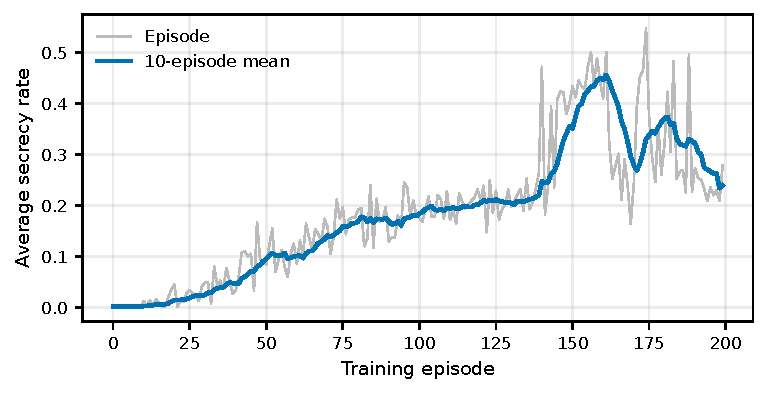
\includegraphics[width=0.98\linewidth]{ppo_training_curve.pdf}
\caption{PPO training curve from \texttt{drl\_ppo\_200ep\_5seed\_stress\_holdoutfit/training\_log.csv}. The smoothed curve shows the 10-episode moving average.}
\label{fig:ppo_training}
\end{figure}

\subsection{Strengthening and ablation suite}

Table~\ref{tab:ablation} and Figure~\ref{fig:strengthening} report the stress holdout-fitted strengthening suite. The oracle-state rollout achieves the best result, with secrecy rate 1.3121 and outage 0.0292, and is treated as an upper reference rather than a deployable method. Among deployable methods, \texttt{rollout\_joint} is strongest. It improves over \texttt{rollout\_fixed\_periodic} by 0.0408 in secrecy rate and reduces outage from 0.5396 to 0.4083, showing that adaptive synchronization contributes beyond rollout motion and power search. It also substantially outperforms \texttt{no\_twin} and \texttt{rollout\_no\_sync}, confirming that twin prediction and synchronization are both important.

\begin{table*}[t]
\centering
\caption{Stress holdout-fitted strengthening suite from \texttt{strengthening\_suite\_3seed\_stress\_holdoutfit/main\_table.csv}.}
\label{tab:ablation}
\begin{tabular}{lrrrr}
\toprule
Method & Runs & Secrecy rate & Outage & Runtime ms/slot \\
\midrule
oracle\_sync & 3 & 1.3121 & 0.0292 & 1412.94 \\
rollout\_joint & 3 & 1.2550 & 0.4083 & 1305.39 \\
rollout\_fixed\_periodic & 3 & 1.2142 & 0.5396 & 1208.12 \\
periodic & 3 & 1.0210 & 0.6417 & 98.84 \\
no\_twin & 3 & 0.9597 & 0.7021 & 1247.44 \\
rollout\_no\_sync & 3 & 0.6670 & 0.8229 & 775.95 \\
sca\_twin & 3 & 0.4708 & 0.8208 & 247.08 \\
random\_budgeted & 3 & 0.0046 & 1.0000 & 6.30 \\
\bottomrule
\end{tabular}
\end{table*}

\begin{figure*}[t]
\centering
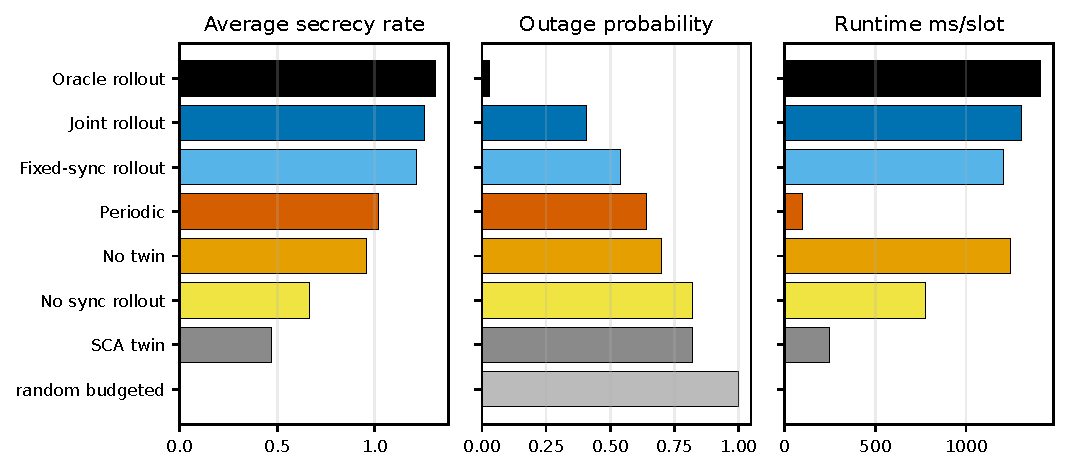
\includegraphics[width=0.96\textwidth]{stress_strengthening_suite.pdf}
\caption{Stress-scenario strengthening suite. The proposed method is below the oracle-state upper reference but outperforms the deployable ablations in secrecy rate and outage.}
\label{fig:strengthening}
\end{figure*}

\subsection{Small exact-DP sanity check}

To verify the dynamic-programming evaluation chain, we also run a deliberately small exact-DP instance. The configuration evaluates 56,784 abstract states and 72 actions over an episode length of 4, obtaining optimal cumulative secrecy 9.5134 and optimal average secrecy 2.3783. Figure~\ref{fig:small_mdp} shows the resulting optimal trace. This experiment is not a paper-scale upper bound because its horizon, action space, and abstraction differ from the main scenarios. Its purpose is to confirm that the exact-DP machinery works on a small instance.

\begin{figure}[t]
\centering
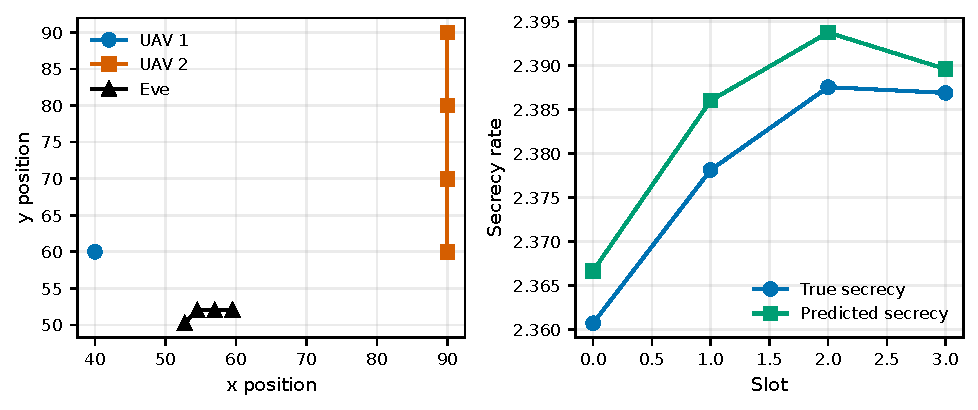
\includegraphics[width=0.98\linewidth]{small_mdp_trace.pdf}
\caption{Small exact-DP sanity-check trace from \texttt{small\_mdp\_bound/optimal\_trace.csv}.}
\label{fig:small_mdp}
\end{figure}

\subsection{Runtime tradeoff}

The main limitation of the proposed method is runtime. In the main 20-seed table, \texttt{rollout\_joint} requires approximately 1265.75, 1262.04, and 1295.63 ms/slot in the base, hard, and stress scenarios, respectively. The corresponding \texttt{periodic} runtimes are about 99.65, 97.89, and 98.54 ms/slot. Thus, the proposed method is better interpreted as a performance-oriented controller for edge-assisted or moderate-timescale decision making, rather than as an ultra-low-latency onboard controller in its current implementation.

\section{Discussion}
\label{sec:discussion}

\subsection{Interpretation of the main claim}

The experiments support a focused claim: in the evaluated simulator, secrecy-aware synchronization should be optimized jointly with UAV motion, source power, and cooperative jamming. The evidence is strongest in the calibrated stress scenario, where stale or low-quality twin information has a visible effect on outage. In that setting, \texttt{rollout\_joint} improves both average secrecy rate and outage relative to periodic, risk-triggered, and margin-triggered rules.

The base scenario should be interpreted more cautiously. Although \texttt{rollout\_joint} has the highest average secrecy rate, its outage probability is the same as \texttt{periodic}. This means the base case demonstrates competitiveness and modest secrecy gain rather than a major reliability improvement. The hard scenario sits between these two regimes. This pattern is scientifically useful because it shows that the proposed method is most valuable when synchronization quality and outage risk are actually limiting factors.

\subsection{Why the oracle and ablation results matter}

The oracle-state rollout establishes that better eavesdropper state information can substantially reduce outage. The gap between \texttt{oracle\_sync} and \texttt{rollout\_joint} therefore quantifies remaining room for improvement in twin accuracy, synchronization reliability, and control approximation. The \texttt{rollout\_fixed\_periodic} result is also important: it uses rollout search but removes adaptive synchronization. Its weaker performance indicates that the proposed gain is not only caused by better motion and power search. The \texttt{rollout\_no\_sync} and \texttt{no\_twin} results further show that neither stale-state rollout nor twin-free control is sufficient in the stress scenario.

\subsection{Scope of the certificate}

The certificate improves the scientific structure of the paper because it prevents the controller from relying blindly on twin-predicted secrecy. The holdout validation results show that the fitted upper bound is conservative on the evaluated trajectories. Nevertheless, the certificate is empirical and policy-dependent. It should be described as an in-policy risk estimator, not as a formal proof of safety for all possible eavesdropper behaviors. A stronger future version would test distribution shift explicitly, for example by changing Eve mobility, channel parameters, synchronization failure probability, and user layouts after calibration.

\subsection{Limitations}

The study has four main limitations. First, the simulator abstracts many real-world effects, including sensing errors, UAV dynamics, regulatory constraints, and hardware-level communication overhead. Second, the rollout controller is computationally expensive, requiring about 1.2--1.3 seconds per slot in the main experiments. Third, the PPO baseline uses a limited 200-episode training budget and should be treated only as a lightweight comparison. Fourth, the exact-DP experiment is a sanity check on a reduced model, not a global optimality certificate for the paper-scale scenarios.

These limitations do not invalidate the main result, but they define the appropriate strength of the paper's claims. The work is best positioned as a simulation-based communication-system study showing the value of jointly optimizing digital-twin synchronization and physical-layer security control.

\subsection{Future work}

Future work should reduce runtime through parallel rollout evaluation, learned value approximators, candidate pruning, and adaptive horizon selection. The certificate should be extended to explicit distribution-shift validation and possibly to stronger conformal-style coverage conditions. Larger networks with more UAVs, multiple eavesdroppers, and richer channel dynamics should also be studied. Finally, reinforcement-learning baselines should be revisited with larger training budgets and architectures designed specifically for the coupled synchronization-control action space.

\section{Conclusion}
\label{sec:conclusion}

This paper investigated secure UAV communication with digital-twin uncertainty and limited synchronization resources. We formulated a joint synchronization and control problem in which two cooperative UAVs select synchronization bandwidth, motion, source power, and jamming power while serving ground users in the presence of a mobile eavesdropper. We proposed an empirical-risk-aware joint rollout controller and validated a holdout-fitted secrecy-loss risk estimator.

The final results support the value of joint synchronization-control design. At the calibrated non-saturated stress threshold, the proposed controller improves average secrecy rate over periodic synchronization by 0.2683 and reduces secrecy outage by 0.2141. A stress-threshold sweep shows that the secrecy-rate gain is stable across the tested $R_{\min}$ values, while outage reduction is most meaningful within the informative non-saturated threshold range. Additional stress-scenario experiments show that it outperforms SCA baselines, no-twin rollout, no-synchronization rollout, and fixed-period rollout, while remaining below an oracle-state upper reference. A lightweight PPO diagnostic run did not learn a competitive policy within 200 episodes, so stronger DRL comparisons remain future work. The risk-estimator validation results show empirical cover rates above the diagnostic 0.95 target on the evaluated holdout groups.

The method is not yet a low-latency onboard solution because its rollout search is computationally expensive. The risk estimator is also empirical and should be recalibrated under major distribution shifts. Even with these limitations, the study provides evidence that digital-twin synchronization should be treated as an active security-control variable rather than as a fixed background maintenance process.


\bmsubsection*{Conflict of Interest Statement}
The authors declare no conflicts of interest.

\bmsubsection*{Data Availability Statement}
The simulation code, configurations, and result tables are maintained in the project repository. The numerical values reported in this manuscript are derived from the result files under \texttt{results/final\_2026-05-12/}.

\bibliography{refs}

\end{document}
